%% LyX 2.1.3 created this file.  For more info, see http://www.lyx.org/.
%% Do not edit unless you really know what you are doing.
\documentclass[english,hyperref={bookmarks=false}]{beamer}
\usepackage{booktabs}
\usepackage[T1]{fontenc}
\usepackage[latin9]{inputenc}
\setcounter{secnumdepth}{3}
\setcounter{tocdepth}{3}
\usepackage{comment}
\usepackage{babel}
\usepackage{url}
\usepackage{graphicx}
\ifx\hypersetup\undefined
  \AtBeginDocument{%
    \hypersetup{unicode=true,pdfusetitle,
 bookmarks=false,
 breaklinks=false,pdfborder={0 0 0},backref=false,colorlinks=true}
  }
\else
  \hypersetup{unicode=true,pdfusetitle,
 bookmarks=false,
 breaklinks=false,pdfborder={0 0 0},backref=false,colorlinks=true}
\fi

\makeatletter

%%%%%%%%%%%%%%%%%%%%%%%%%%%%%% LyX specific LaTeX commands.
\newcommand{\noun}[1]{\textsc{#1}}
%% A simple dot to overcome graphicx limitations
\newcommand{\lyxdot}{.}


%%%%%%%%%%%%%%%%%%%%%%%%%%%%%% Textclass specific LaTeX commands.
 % this default might be overridden by plain title style
 \newcommand\makebeamertitle{\frame{\maketitle}}%
 % (ERT) argument for the TOC
 \AtBeginDocument{%
   \let\origtableofcontents=\tableofcontents
   \def\tableofcontents{\@ifnextchar[{\origtableofcontents}{\gobbletableofcontents}}
   \def\gobbletableofcontents#1{\origtableofcontents}
 }

%%%%%%%%%%%%%%%%%%%%%%%%%%%%%% User specified LaTeX commands.
\usetheme{Berkeley}

\makeatother

\begin{document}
\setbeamercolor{background canvas}{bg=}


\title{Biosecurity for Guam in the New Millennium}
\subtitle{Are We More Secure?}


\author{Aubrey Moore}


\institute{{\small{}University of Guam}\\
{\small{}College of Natural and Applied Sciences}\\
{\small{}Cooperative Extension Services / Western Pacific Research
Center}}


\date{Pacific Entomology Conference\\April 2015}

\makebeamertitle

\section*{Introduction}
\begin{frame}{Abstract}


Guam, a transportation hub for the western Pacific, has long been
recognized as a stepping stone for island-hopping invasive insect
species. The frequency of insect pest incursions on Guam has increased
significantly during the past decade, coinciding with major changes
to Guam's biosecurity infrastructure which include establishment of
a USDA-APHIS Plant Inspection Station and transfer of Guam's plant
protection and quarantine officers from the Guam Department of Agriculture
to the Guam Customs and Quarantine Agency. Impacts of these changes
and recent attempts to improve Guam's biosecurity will be discussed.
\end{frame}

\begin{frame}{Where is Guam?}


\begin{center}
\includegraphics[width=0.95\textwidth,height=0.95\textheight,keepaspectratio]{images/Micronesian_Cultural_Area_dot}
\par\end{center}

\end{frame}

\begin{frame}{Challenges}

\begin{itemize}
\item Limited taxonomic expertise

\begin{itemize}
\item only 3 active PhD level entomologists in all of Micronesia (Russ Campbell,
Ross Miller, Aubrey Moore)
\end{itemize}
\item High endemism (about 45\%); many undescribed species
\item Very high introduction rate for alien insects
\end{itemize}
\end{frame}

\begin{frame}{Origin of New Insects on Guam}
\includegraphics[scale=0.4,page=14]{images/GuamInvasiveInsectsMBP20100120.pdf}
\end{frame}

\begin{frame}{Origin of New Insects on Guam (1945-1989)}
\begin{center}
\includegraphics[scale=0.4]{images/pie}
\par\end{center}
Data source: \cite{Schreiner1991}
\end{frame}

\begin{frame}{Current Invasions}

\begin{itemize}
\item Asian cycad scale, \emph{Aulacaspis yasumatsui} - detected 2003; has
killed 90\% of Guam's endemic cycad which was Guam's most populous
tree
\item Coconut rhinoceros beetle, \emph{Oryctes rhinoceros} - detected 2007;
is killing coconut palms, which was Guam's second most populous tree
\item Little fire ant, \emph{Wasmania auropunctata} - detected 2011
\end{itemize}
\end{frame}

\begin{comment}
\begin{frame}{15 new island records in 2010-2011}
\begin{itemize}
\item 4 bark beetles, Scolytidae, from a single CBB trap at a single location 
\item 2 biting flies: a black fly and an anopheline mosquito 
\item little fire ant
\item 8 other species
\end{itemize}
\end{frame}
\end{comment}

\begin{frame}{Early Concerns}
\begin{center}
\includegraphics[width=0.95\textwidth,height=0.95\textheight,keepaspectratio]{images/PanAmClipper1.jpeg}
\par\end{center}

\end{frame}

\begin{frame}{1936 Entomological Survey of Guam}

\begin{itemize}
\item Sponsored by the Hawaiian Sugar Planters Association
\item Results reported in:

\begin{itemize}
\item Sweezey, O. H. 1942. Insects of Guam - 1. Bernice P. Bishop Museum
Bulletin 172 1\textendash 218.\cite{Swezey1942}
\item Sweezey, O. H. 1946. Insects of Guam - 1. Bernice P. Bishop Museum
Bulletin 172 1\textendash 218.\cite{Swezey1946}
\item Gressitt, J.L. 1954 - present. Insects of Micronesia series.\\
\url{http://hbs.bishopmuseum.org/pubs-online/iom.html}
\end{itemize}
\end{itemize}
\end{frame}

\begin{frame}{1936 Entomological Survey of Guam}


Justification for the Survey \cite{Swezey1942}:\medskip{}



\textquotedbl{}Guam is the most important station between the Philippines
and Honolulu on the route of the Pan-American Airways across the Pacific,
and as knowledge of the Guam insect fauna was meager, it was deemed
important to acquire as complete a knowledge as possible of this fauna.
Unknown insects were already being found in planes arriving at Pearl
Harbor, Oahu, and, in spite of the system employed in the fumigation
of the planes, an occasional insect was found which had not fully
succumbed. There was some concern lest unknown pests might survive
and succeed in becoming established, and, perhaps, destructive to
sugar cane and other crops grown in Hawaii.\textquotedbl{}

\end{frame}

\begin{frame}{1936 Entomological Survey of Guam}

\begin{itemize}
\item The 1936 survey identified 50 agricultural pests on Guam which were
not present in Hawaii at the time. 
\item \textquotedbl{}No doubt there are many among them which would become
serious crop pests if they should reach Hawaii and become established.\textquotedbl{}
\cite{Swezey1942}
\end{itemize}
\end{frame}



\begin{comment}

\section*{Suspects}
\begin{frame}{Insects Suspected of being Introduced from Guam or Other Mariana Islands
to Hawaii}

\begin{itemize}
\item Island Hoppers

\begin{itemize}
\item Oriental fruit fly
\item Banana leaf roller
\item Southern green stink bug
\item Grass bagworm
\item Oriental flower beetle
\end{itemize}
\item Endemics

\begin{itemize}
\item Hibiscus whitefly
\item Ochrosia fruit fly
\item Biting bug
\end{itemize}
\end{itemize}
\end{frame}

\begin{frame}{Oriental fruit fly, \emph{Bactrocera dorsalis}}


\textquotedbl{}As much troop and other military movement occurred
about this time between Hawaii and Saipan, where the fly occurred,
this new pest could have come from the latter island.\textquotedbl{}
\cite{Pemberton1964}


\begin{center}
\includegraphics[width=1\textwidth,height=0.5\textheight,keepaspectratio]{images/800px-Bactrocera_dorsalis}
\par\end{center}


\begin{center}
Photo by Scott Bauer
\par\end{center}

\end{frame}

\begin{frame}{Banana leaf roller, \emph{Erionata thrax}}

\begin{itemize}
\item Oahu (Hickam AFB) Davis and Kawamura 1975

\begin{itemize}
\item PHES 22(1): 21.
\end{itemize}
\end{itemize}

\begin{center}
\includegraphics[width=1\textwidth,height=0.5\textheight,keepaspectratio]{images/800px-Starr_020813-0020_Musa_sp\lyxdot }
\par\end{center}


\begin{center}
Photo by Forrest and Kim Starr
\par\end{center}

\end{frame}

\begin{frame}{Southern green stink bug, \emph{Nezara viridula}}


``As this insect is known in Guam and Samoa but not in California,
it possibly came from one of those islands.'' \cite{Pemberton1964}


\begin{center}
\includegraphics[width=1\textwidth,height=0.5\textheight,keepaspectratio]{images/Nezara_viridula16}
\par\end{center}


\begin{center}
Photo by Russ Ottens, University of Georgia, Bugwood.org
\par\end{center}

\end{frame}

\begin{frame}{Grass bagworm}


\includegraphics[scale=0.4,page=51]{\string"/home/aubreymoore/Documents/16gb stick/Presentations/BioInvasionOfGuamMBP20100119/BioInvasionOfGuamMBP20100119\string".pdf}

\end{frame}

\begin{frame}{Oriental flower beetle }


\includegraphics[scale=0.4,page=50]{\string"/home/aubreymoore/Documents/16gb stick/Presentations/BioInvasionOfGuamMBP20100119/BioInvasionOfGuamMBP20100119\string".pdf}

\end{frame}

\begin{frame}{Endemics}

\begin{itemize}
\item Ochrosia fruit fly, \emph{Bactrocera ochrosiae} (Malloch) 1942 (Diptera:
Tephritidae)

\begin{itemize}
\item Molokai 1972 Kjargaard, PHES 32: 5.
\end{itemize}
\item \emph{Botocudo marianensis} (Usinger) 1946 (Hemiptera: Lygaeidae)

\begin{itemize}
\item Oahu 1974, Beardsley, PHES 22:160-161
\item Maui 1972, Gagne, PHES 22:167
\item Hawaii 1977, Beardsley, PHES 22: 410
\item Kauai 1977, Nakahara, PHES 23(2): 158
\end{itemize}
\end{itemize}
\end{frame}

\end{comment}

\begin{comment}

\section*{Interceptions}
\begin{frame}{Interceptions}


\begin{center}
\includegraphics[width=1\textwidth,height=0.5\textheight,keepaspectratio]{images/washdownManual}
\par\end{center}


\begin{center}
{\tiny{}\url{http://www.afpmb.org/sites/default/files/pubs/techguides/tg31.pdf}}
\par\end{center}{\tiny \par}


\begin{center}
\medskip{}
Appendix J - USDA APHIS History of Interceptions
\par\end{center}


\begin{center}
{\tiny{}\url{http://www.afpmb.org/sites/default/files/pubs/techguides/tg31/appendix-j.xls}}
\par\end{center}{\tiny \par}

\end{frame}

\begin{frame}[allowframebreaks]{APHIS Interceptions on USAF Aircraft Arriving in Honolulu from Guam}

\begin{itemize}
\item COLEOPTERA

\begin{itemize}
\item Curculionidae 

\begin{itemize}
\item \emph{Myllocerus} sp. (10/27/1987; 6/10/1986) 
\end{itemize}
\item Elateridae 

\begin{itemize}
\item \emph{Conoderus} sp. (6/11/1989) 
\end{itemize}
\item Chrysomelidae 

\begin{itemize}
\item \emph{Altica} sp. (10/11/1984) 
\item \emph{Rhyparida} sp. (10/18/1984) 
\end{itemize}
\item Scarabeidae 

\begin{itemize}
\item \emph{Adoretus sinicus} (8/28/1987; 4/1/1990; 7/29/1990) 
\item \emph{Anomola} sp. (11/27/1986; 8/20/1987; 6/14/1985; 5/16/1990; 5/12/1989;
6/8/1992; 6/11/1990; 5/25/1991) 
\item \emph{Popillia lewisi} (7/22/1991; 8/2/1991; 6/8/1990) 
\item \emph{Protaetia orientalis} (11/22/1984; 5/10/1993) 
\end{itemize}
\item Tenebrionidae 

\begin{itemize}
\item \emph{Caedius} sp. (7/2/1990; 6/9/1990; 6/9/1990) 
\item \emph{Gonocephalum} sp. (4/8/1990; 6/15/1990; 6/15/1990) 
\end{itemize}
\end{itemize}
\item LEPIDOPTERA

\begin{itemize}
\item Noctuidae 

\begin{itemize}
\item unidentified sp. (9/18/1987; 11/30/1984; 9/17/1989; 9/17/1989) 
\item \emph{Chrysodeixis chalcites} (11/11/1984) NKFG 
\item \emph{Helicoverpa armigera} (4/6/1986) 
\item \emph{Leucania} sp. (8/30/1987; 12/14/1985) 
\item \emph{Mocis frugalis} (9/18/1987; 7/6/1990) 
\item \emph{Platysenta} sp. (10/23/1986; 8/16/1987; 8/31/1987; 12/11/1984;
11/7/1984) NKFG 
\item \emph{Pseudaletia} sp. (9/4/1987; 3/31/1990) 
\item \emph{Spodoptera} sp. (4/21/1987; 9/20/1987; 5/9/1987; 8/17/1987;
7/10/1987; 12/14/1985; 8/28/1993; 6/29/1989; 6/30/1990) 
\item \emph{Spodoptera litura} (1/29/1985; 11/30/1984; 10/6/1984; 8/5/1986) 
\item \emph{Spodoptera mauritia} (8/24/1987; 3/5/1986) 
\end{itemize}
\item Pyralidae

\begin{itemize}
\item Unidentified sp. (9/2/1987; 9/14/1987) 
\item \emph{Cnaphalocrocis medinalis} (5/17/1987;9/20/1985; 9/15/1984; 10/6/1984;
10/23/1984) NKFG
\item \emph{Herpetogramma licarsisalis} (8/22/1984) 
\item \emph{Ostrinia furnacalis} (9/15/1984) 
\item \emph{Sameodes cancellalis} (11/27/1984) NKFG 
\end{itemize}
\item Lyonetiidae 

\begin{itemize}
\item Unidentified sp. (7/30/1985) NKFG 
\end{itemize}
\item Sphingidae 

\begin{itemize}
\item Unidentified species (11/24/1987) 
\end{itemize}
\end{itemize}
\item HEMIPTERA

\begin{itemize}
\item Cydnidae 

\begin{itemize}
\item \emph{Aethus indicus} (7/13/1990) NKFG 
\end{itemize}
\item Pentatomidae 

\begin{itemize}
\item \emph{Plautia} sp. (7/2/1985) NKFG
\end{itemize}
\item Cicadellidae 

\begin{itemize}
\item Unidentified sp. (6/6/1987; 6/16/1990) 
\end{itemize}
\end{itemize}
\item ISOPTERA

\begin{itemize}
\item Rhinotermitidae 

\begin{itemize}
\item \emph{Coptotermes} sp. (5/24/1990)
\end{itemize}
\end{itemize}
\item ORTHOPTERA

\begin{itemize}
\item Tettigoniidae 

\begin{itemize}
\item \emph{Euconocephalus} sp.(11/22/1987; 11/30/1987; 10/30/1987; 9/11/1987;
10/16/1987; 12/15/1984; 1/15/1986) 
\end{itemize}
\item Gryllidae 

\begin{itemize}
\item \emph{Metioche vittaticollis} (8/3/1986) (listed in MAD as \emph{Trigonidium
vittaticolis}) 
\item \emph{Phyllopalpus} sp. (8/30/1987) NKFG 
\end{itemize}
\end{itemize}
\item HYMENOPTERA

\begin{itemize}
\item Torymidae 

\begin{itemize}
\item \emph{Megastigmus pistaciae} (1/14/1985) NKFG 
\end{itemize}
\end{itemize}
\end{itemize}
\end{frame}

\begin{frame}{Interceptions of Insects on USAF Aircraft Arriving on Guam}


\begin{center}
\noun{NO RECORDS AVAILABLE}
\par\end{center}


\begin{center}
\includegraphics[scale=0.3]{images/Smiley}
\par\end{center}

\end{frame}

\section*{Why is Guam Such a Good Source?}
\begin{frame}{Why is Guam Such a Good Source?}

\begin{itemize}
\item Guam's biosecurity is weak 
\item Guam is hypersusceptable to pest invasions and outbreaks 
\item Agricultural pests may remain hidden on Guam
\item Active military pathway for movement of invasive species between Guam
and Hawaii
\end{itemize}
\end{frame}

\begin{frame}{Why is Guam Such a Good Source?}


\framesubtitle{Guam's biosecurity is Weak}
\begin{itemize}
\item 2003 - USDA APHIS establishes the Guam Plant Inspection Station

\begin{itemize}
\item 0 APHIS inspectors; 0 identifiers
\end{itemize}
\item 2003 - GovGuam PPQ inspectors moved from Agriculture to Customs
\item Intercepted insects are usually identified only to taxonomic level
of order or family
\item Double standard for treatment

\begin{itemize}
\item Infested plant material from US or trans-shipped through the US is
``reconditioned'' (washed with soapy water)
\item Infested plant material from elsewhere is destroyed
\end{itemize}
\end{itemize}
\end{frame}

\begin{frame}{Why is Guam Such a Good Source?}


\framesubtitle{Guam is hypersusceptable to pest invasions and outbreaks}


\begin{center}
\includegraphics[scale=0.2]{images/bts}
\par\end{center}


All tropical islands are susceptible to biological invasions and outbreaks.
\begin{itemize}
\item Guam is hypersusceptable because:

\begin{itemize}
\item the brown treesnake has exterminated birds and other vertebrate insectivores

\begin{itemize}
\item large day-flying insects are extremely abundant
\end{itemize}
\end{itemize}
\item Guam does not have a large guild of previously imported biocontrol
agents, as does Hawaii
\end{itemize}
\end{frame}

\end{comment}

\begin{frame}{Why is Guam Such a Good Source?}


\framesubtitle{Agricultural pests may remain hidden on Guam}
\begin{itemize}
\item Guam has no large-scale commercial farming and limited variety of
crops. Agricultural pests may be overlooked because their hosts are
not grown as crops on Guam.
\item Examples:

\begin{itemize}
\item coffee berry borer, \emph{Hypothenemus hampei} (Coleoptera: Scolytidae)

\begin{itemize}
\item Saipan 1944 Dybas; Pohnpei 1953 Gressitt; Pohnpei 1950 Adams \cite{Wood1960}
\end{itemize}
\item sugarcane leafmining buprestid, \emph{Aphanisticus cochinchinae seminulum}
Obenberger (Coleoptera: Buprestidae)

\begin{itemize}
\item Guam 2007\cite{Zack2009}
\end{itemize}
\end{itemize}
\end{itemize}
\end{frame}

\begin{frame}{Why is Guam Such a Good Source?}


\framesubtitle{Active military pathway for movement of invasive species between
Guam and Hawaii}
\begin{itemize}
\item There is ample historical evidence that several pest insects have
moved from Guam to Hawaii in association with movements of military
personnel and equipment. 
\item It is expected that traffic of invasion species on this ``military
pathway'' will increase as the Guam military buildup gets underway.
\end{itemize}
\end{frame}

\section*{2004 Changes}

\begin{frame}{Changes}
\framesubtitle{Guam PPQ Officers Transfered from Ag to Customs}
In November 2004, the duties and functions of plant protection
and quarantine were transferred from the Department of Agriculture
to the Customs and Quarantine Agency of Guam. However, two (2)
Plant Protection and Quarantine Officers, later re-designated and
assigned the title of "Commodity Inspectors"
and one (1) Entomologist, remained with the Department of Agriculture to manage and operate the USDA/Guam Plant Inspection Station. The duties of border inspection and various inland quarantine duties,
including, but not limited to, store inspections, smuggling and
interdiction, invasive species control and management, federal
fumigations, federal export certifications, local export certifications,
eradication program management, and local and federal monitoring
program management, were left as responsibilities of the Department
of Agriculture. \cite{Respicio2009}
\end{frame}

\begin{frame}{Changes}
\framesubtitle{Establishment of the USDA APHIS Guam Plant Inspection Station}
We are amending the regulations governing the importation of nursery stock and other articles by designating the ports of Atlanta, Georgia, and Agana, Guam, as plant inspection stations. The addition of the two plant inspection stations will help reduce transportation time and costs to importers who must currently import plants through inspection stations that are considerably distant from the importers' facilities. \cite{FR2003}
\end{frame}

\begin{frame}{Number of Guam Invertebrate Interceptions During 2014}
\framesubtitle{0.6 interceptions per day}
\begin{enumerate}
\item Aphids: 38
\item Araneae (spiders): 38
\item Thrips: 32
\item Collembola: 20
\item Diptera: 20
\item Coleoptera: 20
\item Disease Symptoms: 10
\item Heteroptera: 10
\item Lepidoptera: 10
\item Mites: 10
\item Snails and Slugs: 9
\item Psocoptera: 5
\item Earwigs: 5
\item Hymenoptera: 3
\item Mealybugs: 3
\end{enumerate}
\end{frame}

\begin{frame}{Guam's Interception Rate Compared to Hawaii's}
\begin{center}
\begin{tabular}{p{2in}r} 
\toprule 
Location & Interceptions per day \\ 
\midrule 
Guam 2014 & 0.6 \\ 
Hawaii State (1995-2001) & 2.1 \\ 
Kahului Airport Risk Assessment (2000-2001) & 10.8 \\
\bottomrule 
\end{tabular}
\end{center}
\end{frame}

%\begin{comment}
\begin{frame}{New Island Records in the Decade prior to 2004 Changes (1995-2004)}
\begin{enumerate}
\item 2000 EULOPHIDAE \textit{Thripobius semiluteus}
\item 2000 BDELLIDAE \textit{Bdella distincta}
\item 2002 PSEUDOCOCCIDAE \textit{Paracoccus marginatus}
\item 2002 TETRANYCHIDAE \textit{Eotetranychus sexmaculatus}
\item 2003 DIASPIDIDAE \textit{Aulacaspis yasumatsui}
\item 2003 ORTHEZIDAE \textit{Orthezia insignis (unconfirmed)}
\item 2003 TINEIDAE \textit{Erechthisa sp.}
\item 2003 DIASPIDIDAE \textit{Pseudaulacaspis cockerelli}
\item 2004 PSEUDOCOCCIDAE \textit{Nipaecoccus nipae}
\item 2004 ALEYRODIDAE \textit{Metaleurodes cardini}
\end{enumerate}
\end{frame}
%\end{comment}

\begin{frame}[allowframebreaks]{New Island Records in the Decade after 2004 Changes (2005-2014)}
\begin{enumerate}
\item 2005 SPHINGIDAE \textit{Daphnis nerii}
\item 2005 TINEIDAE \textit{Dasyses rugosella}
\item 2005 COSMOPTERIGIDAE \textit{Anatrychintis sp.}
\item 2006 EULOPHIDAE \textit{Quadrastichus erythrinae}
\item 2006 FORMICIDAE \textit{Lepisiota frauenfeldi}
\item 2007 ALEURIDAE \textit{Tetraleurodes acaciae}
\item 2007 COCCINELLIDAE \textit{Epilachna cucrubitae}
\item 2007 PSYLLIDAE \textit{Diaphorina citri}
\item 2007 SCARABAEIDAE \textit{Oryctes rhinoceros}
\item 2009 BUPRESTIDAE \textit{Aphanisticus cochinchinae}
\item 2009 EULOPHIDAE \textit{Selittrichoides casuarinae}
\item 2010 CERATOPOGONIDAE \textit{Culicoides peliliouensis}
\item 2010 CERATOPOGONIDAE \textit{Dasyhelia carolinensis}
\item 2010 CERATOPOGONIDAE \textit{Dasyhelea dupliforceps}
\item 2010 CYDNIDAE \textit{Byrsinus varians}
\item 2010 CYDNIDAE \textit{Fromundus biimpressus}
\item 2010 CYDNIDAE \textit{Rhytidoporus indentatus}
\item 2010 TERMITIDAE \textit{Nasutitermes luzonicus}
\item 2010 TERMITIDAE \textit{Schederorhinotermes longirostris}
\item 2010 ARANAEIDAE \textit{Araneus ventricosus}
\item 2010 CULICIDAE \textit{Anopheles campestris}
\item 2011 SCOLYTIDAE \textit{Coccotrypes advena}
\item 2011 SCOLYTIDAE \textit{Hypothemus burmanus}
\item 2011 SCOLYTIDAE \textit{Hypothemus crudiae}
\item 2011 SCOLYTIDAE \textit{Xylosandrus crassiusculus}
\item 2011 CULICIDAE \textit{Anopheles aureohirtum}
\item 2011 HESPERIIDAE \textit{species needed}
\item 2011 ALEYRODIDAE \textit{Dialeuropora decempunctata}
\item 2011 COCCIDAE \textit{Pulvinaria urbicola}
\item 2011 FORMICIDAE \textit{Wasmannia auropunctata}
\item 2011 TENUIPALPIDAE \textit{Brevipalpus californicus}
\item 2011 CUNAXIDAE \textit{Cunaxa sp.}
\item 2011 EUPODIDAE \textit{Eupodes sp.}
\item 2011 PHYTOSEIDAE \textit{Amblyscius obtusus species group A. nr lentiginosus}
\item 2011 ERIOPHYIDAE \textit{Acerimina tiliaceae}
\item 2011 GLYCIPHAGIDAE \textit{Lepidoglyphus destructor}
\item 2012 FORMICIDAE \textit{Polyrachis sp. (not dives)}
\item 2012 THRIPIDAE \textit{Dinurothrips hookeri}
\item 2013 PSEUDOCOCCIDAE \textit{Cocoidohystrix insolita}
\item 2014 PENTATOMIDAE \textit{Halymorpha halys}
\item 2014 DIASPIDIDAE \textit{Pseudaonidia duplex}
\item 2014 CHRYSOMELIDAE \textit{Diabrotica undecimpuntata}
\item 2014 VARROIDAE \textit{Varroa destructor}
\end{enumerate}
\end{frame}

\section*{Attempts at Improvement}

\begin{frame}{Attempts to Improve Guam's Biosecurity}
\begin{itemize}
\item GISAC
\item GISC
\item National Plant Diagnostics Network - First Detector Training
\item Annual APHIS/SPC Training for Micronesian PPQ Officers
\end{itemize}
\end{frame}

\begin{frame}{Attempts to Improve Guam's Biosecurity}
\begin{itemize}
\item Guam Department of Agriculture Biosecurity Division

\end{itemize}
\end{frame}

\begin{frame}{Attempts to Improve Guam's Biosecurity}
\begin{itemize}
\item Micronesia Biosecurity Plan
\end{itemize}
\end{frame}

\section*{Conclusions}
\begin{frame}{Conclusions}

\begin{itemize}
\item Evidence indicates that Guam has been and continues to be a high risk
source of insects invading Hawaii.
\end{itemize}

\end{frame}

\section*{References}
\begin{frame}[allowframebreaks]{References}


\bibliographystyle{plainnat}
\bibliography{GuamHawaiiBugConnection}



\end{frame}

\end{document}
